\documentclass[12pt,a4paper]{report}

% ===== PACKAGES =====
\usepackage[utf8]{inputenc}
\usepackage{amsmath}
\usepackage{amssymb}
\usepackage{graphicx}
\usepackage{hyperref}
\usepackage{geometry}
\usepackage{fancyhdr}
\usepackage{titlesec}
\usepackage{float}
\usepackage{caption}
\usepackage{listings}
\usepackage[usenames]{color}
\usepackage{enumitem}
\usepackage{tikz}
\usetikzlibrary{positioning}

% ===== SETTINGS =====
\geometry{left=3cm,right=2.5cm,top=2.5cm,bottom=2.5cm}
\setlength{\headheight}{14.5pt}
\pagestyle{fancy}
\fancyhf{}
\rhead{\thepage}
\lhead{SeatSurfer Thesis}

\begin{document}

% ===== TITLE PAGE =====
\begin{titlepage}
    \centering
    % \includegraphics[width=0.2\textwidth]{ubb_logo.png}\par\vspace{1cm}
    \textsc{\LARGE Babeș-Bolyai University}\\[0.5cm]
    \textsc{\Large Faculty of Mathematics and Computer Science}\\[1.5cm]

    {\huge\bfseries SeatSurfer: A Database-Centric Seat Management System\\[0.4cm]}

    \vspace{1.5cm}
    \Large
    \textbf{Bachelor’s Thesis}\\[0.5cm]

    \begin{flushleft}
        \textbf{Author:} Your Name Here\\
        \textbf{Supervisor:} Lect. Dr. [Supervisor Name] \\
        \textbf{Specialization:} Computer Science (English) \\
        \textbf{Year:} 2025
    \end{flushleft}

    \vfill
\end{titlepage}

% ===== ABSTRACT =====
\chapter*{Abstract}
\addcontentsline{toc}{chapter}{Abstract}

SeatSurfer is a modern web and mobile application designed to address the rising need for flexible and efficient seat management in office environments. The system allows employees to book seats in real time, view floor layouts, and manage reservations. Admins can configure office layouts, generate occupancy reports, and analyze usage patterns.

This thesis presents the theoretical and practical underpinnings of database systems applied in the development of SeatSurfer. We explore existing systems, compare architectural choices, and present the technologies used — including Flutter, Spring Boot, PostgreSQL, and Firebase. A relational data model was chosen to enable fast queries, maintain data integrity, and support multi-user interaction.

The development process follows Agile methodology with continuous integration and testing, ensuring modularity, scalability, and maintainability. The final product provides a robust infrastructure for seat reservation, occupancy analytics, and real-time collaboration between employees and administrators.

\vspace{0.5cm}
\noindent \textbf{Keywords:} databases, seat booking, Flutter, Spring Boot, reservation system, PostgreSQL, office management.

\newpage

% ===== TABLE OF CONTENTS =====
\tableofcontents
\newpage

% ===== CHAPTER 1 =====
\chapter{Introduction}

\section{Context and Motivation}
With the growing trend of hybrid and flexible work models, managing physical office spaces efficiently has become a new challenge. Organizations are looking for smart systems that offer visibility over seat occupancy and enable employees to plan their presence in shared environments. The SeatSurfer application addresses this demand by providing a seat reservation platform integrated with real-time data and analytics.

\section{Purpose and Scope}
The primary goal of this thesis is to present a practical and theoretical analysis of database systems applied to a real-world use case: SeatSurfer. The application allows users to view floor layouts, reserve seats, manage bookings, and generate occupancy reports.

From a technical perspective, the project focuses on:
\begin{itemize}
    \item Designing an optimized relational data model
    \item Implementing a RESTful backend service using Spring Boot
    \item Building an intuitive frontend in Flutter
    \item Integrating user authentication and secure booking workflows
    \item Creating admin dashboards with occupancy insights
\end{itemize}

\section{Structure of the Thesis}
This paper is structured as follows:
\begin{itemize}
    \item \textbf{Chapter 2} introduces similar systems and applications, discussing their functionalities and limitations.
    \item \textbf{Chapter 3} describes the technologies used in the development of SeatSurfer.
    \item \textbf{Chapter 4} presents the architecture of the system, including database design and API structure.
    \item \textbf{Chapter 5} showcases the functionalities implemented, such as booking, admin tools, analytics, and PDF reports.
    \item \textbf{Chapter 6} concludes the paper and proposes future development directions.
\end{itemize}

% ===== CHAPTER 2 =====
\chapter{Related Work and System Benefits}

\section{Existing Applications and Their Limitations}
Several seat booking and office management platforms have emerged in recent years, such as Microsoft Outlook Room Finder, Robin, Deskbird, and Skedda. These tools help organizations manage office layouts and enable employees to book seats and meeting rooms. However, many existing systems suffer from:
\begin{itemize}
    \item High costs of licensing
    \item Lack of customization
    \item Limited data analytics features
    \item Poor integration with internal tools
\end{itemize}

\section{Innovation Introduced by SeatSurfer}
SeatSurfer introduces:
\begin{itemize}
    \item Full control over seat layouts and logic
    \item Visual seat mapping
    \item Smart PDF reports with date filtering
    \item Integration with Google and Outlook calendars
    \item Open-source and customizable deployment
\end{itemize}

\section{Advantages of the Chosen Stack}
By using Flutter, Spring Boot, PostgreSQL, and Firebase, SeatSurfer provides modular, scalable, and secure architecture suitable for real-time collaboration and future scalability.

\newpage

% ===== CHAPTER 3 =====
\chapter{Technologies Used}

\section{Overview of the Tech Stack}
SeatSurfer’s architecture is based on:
\begin{itemize}
    \item Flutter – frontend UI
    \item Spring Boot – backend API
    \item PostgreSQL – database
    \item Firebase – authentication
\end{itemize}

\section{Flutter: UI Development}
Flutter is an open-source framework by Google that allows cross-platform development from a single codebase \cite{flutter}. With it, SeatSurfer ensures a responsive user experience on Android, iOS, and web using a single codebase.

\section{Spring Boot: Backend Services}
Spring Boot is a powerful Java-based backend framework that simplifies the development of RESTful APIs \cite{springboot}. It enables rapid application development using dependency injection, controller routing, and service-based architecture.

\section{PostgreSQL: Relational Database}
PostgreSQL is an open-source relational database system known for its strong support of transactions, constraints, and indexing \cite{postgresql}. SeatSurfer stores seat, booking, and user data in PostgreSQL using a normalized schema.

\section{Firebase: Authentication and Messaging}
Firebase offers secure authentication and session control for both users and admins \cite{firebase}. It integrates easily with Flutter and provides token-based authentication used by the backend for access control.

\section{Development Tools}
The following tools were used throughout the project:
\begin{itemize}
    \item Visual Studio Code – frontend
    \item IntelliJ IDEA – backend
    \item Postman – API testing
    \item GitHub – version control
\end{itemize}

% =======================
% CHAPTER 4
% =======================
\chapter{System Architecture}

\section{Overview}

The architecture of SeatSurfer follows a layered and modular design to ensure scalability, maintainability, and clarity. The system consists of the following components:
\begin{itemize}
    \item A Flutter-based frontend for mobile and web clients
    \item A Spring Boot REST API backend
    \item A PostgreSQL relational database
    \item Firebase authentication for login and role management
\end{itemize}

Communication between components is stateless and performed via RESTful HTTP endpoints. Booking logic, seat layout logic, and occupancy reporting are handled exclusively on the backend.

\section{Entity-Relationship Diagram}

The core data model is relational and consists of the following entities:
\begin{itemize}
    \item \textbf{User} — a person with an email, role (user/admin), and associated bookings
    \item \textbf{Floor} — a uniquely identified floor layout in a building
    \item \textbf{Seat} — a specific seat on a floor, defined by coordinates
    \item \textbf{Booking} — a user's reservation for a given seat and date
\end{itemize}

\begin{figure}[H]
    \centering
    \begin{tikzpicture}[node distance=2.5cm, every node/.style={draw, minimum height=1.2cm, minimum width=2.8cm}]
        \node (user) {User};
        \node (booking) [right of=user, xshift=4cm] {Booking};
        \node (seat) [below of=booking] {Seat};
        \node (floor) [below of=seat] {Floor};

        \draw[->] (user) -- node[above] {userId} (booking);
        \draw[->] (booking) -- node[right] {seatId} (seat);
        \draw[->] (seat) -- node[right] {floorId} (floor);
    \end{tikzpicture}
    \caption{Entity-Relationship Diagram of the SeatSurfer Database}
    \label{fig:erd}
\end{figure}

This schema is normalized, with foreign key relationships ensuring data consistency. Additional constraints like unique bookings per user per date are enforced at the database level.

\section{Backend Architecture (Spring Boot)}

The backend follows a clean separation of concerns using the standard structure:

\begin{itemize}
    \item \textbf{Controller Layer} — handles incoming HTTP requests
    \item \textbf{Service Layer} — contains business logic
    \item \textbf{Repository Layer} — interacts with the database via Spring Data JPA
\end{itemize}

Each entity (e.g., `Seat`, `Booking`) has its own `Controller`, `Service`, and `Repository`. Example:
\begin{itemize}
    \item `BookingController.java` exposes `/api/bookings`
    \item `BookingService.java` contains logic to prevent double bookings
    \item `BookingRepository.java` provides query methods using JPA
\end{itemize}

\section{Frontend Integration (Flutter)}

The Flutter application interacts with the backend through HTTP REST API calls. Users are authenticated via Firebase, and the access token is sent in the request headers.

The frontend maintains the current session, makes API calls to:
\begin{itemize}
    \item Display available seats per floor/date
    \item Send booking/cancel requests
    \item Display future bookings, occupancy charts
\end{itemize}

\section{System Interaction Diagram}

\begin{figure}[H]
    \centering
    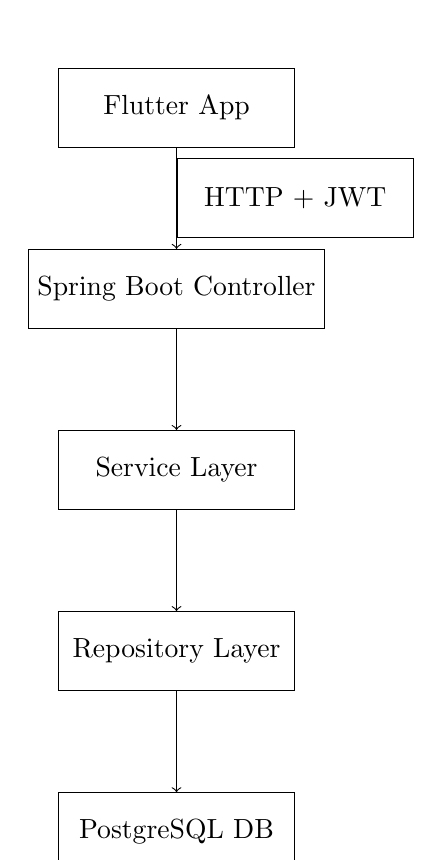
\begin{tikzpicture}[node distance=2.3cm, every node/.style={draw, minimum width=3cm, minimum height=1cm}]
        \node (user) {Flutter App};
        \node (controller) [below of=user] {Spring Boot Controller};
        \node (service) [below of=controller] {Service Layer};
        \node (repo) [below of=service] {Repository Layer};
        \node (db) [below of=repo] {PostgreSQL DB};

        \draw[->] (user) -- node[right] {HTTP + JWT} (controller);
        \draw[->] (controller) -- (service);
        \draw[->] (service) -- (repo);
        \draw[->] (repo) -- (db);
    \end{tikzpicture}
    \caption{System Architecture Flow}
    \label{fig:architecture}
\end{figure}

The design allows each layer to evolve independently. For example, switching from PostgreSQL to MySQL, or adding a caching layer like Redis, would not affect the controller or frontend.

\newpage

% ===== BIBLIOGRAPHY =====
\bibliographystyle{plain}
\bibliography{references}

\end{document}